\documentclass{standalone}

\usepackage{tikz}
\usepackage{amsmath}
\usepackage{unicode-math}
\usepackage{xcolor}
\colorlet{darkRed}{red!40!black}
\colorlet{darkBlue}{cyan!50!black}
\colorlet{darkYellow}{yellow!50!black}


\begin{document}

\usetikzlibrary{calc}

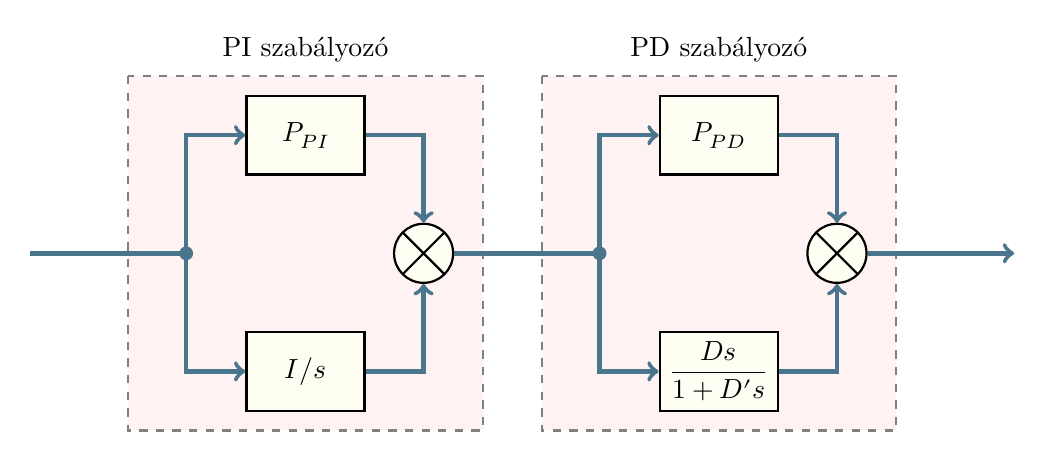
\begin{tikzpicture}[
    thick,
    arr/.style={ultra thick, draw=darkBlue},
    err/.style={ultra thick, draw=darkRed},
    box/.style={
        rectangle,
        minimum width=1.5cm,
        minimum  height=1cm,
        draw=black,
        align=center,
        fill=yellow!5,
      },
    cross/.style={path picture={
            \draw[black]
            (path picture bounding box.south east) -- (path picture bounding box.north west) (path picture bounding
            box.south west)
            -- (path picture bounding box.north east);
          }},
    sum/.style={circle, minimum size=.75cm, draw=black, cross, fill=yellow!5},
    ma/.style={midway, above},
    mb/.style={midway, below},
    ml/.style={midway, left},
  ]
  \draw[gray, dashed, fill=red!5] (0.25,2.25) rectangle (4.75, -2.25);
  \draw[gray, dashed, fill=red!5] (5.50,2.25) rectangle (10.0, -2.25);

  \node[above=-2mm] at (2.50,2.50) {PI szabályozó};
  \node[above=-2mm] at (7.75,2.50) {PD szabályozó};

  \node[box] (P1) at (2.5,+1.5) {$P_{PI}$};
  \node[box] (I1) at (2.5,-1.5) {$I / s$};
  \node[sum] (s1) at (4,0) {};

  \begin{scope}[xshift=5.25cm]
    \node[box] (P2) at (2.5,+1.5) {$P_{PD}$};
    \node[box] (D2) at (2.5,-1.5) {$\dfrac{Ds}{1 + D's}$};
    \node[sum] (s2) at (4,0) {};
  \end{scope}

  \draw[arr, to-] (P1.west) -- ++(-.75,0) |- (-1,0);
  \draw[arr, to-] (I1.west) -- ++(-.75,0) |- (-1,0);
  \draw[arr, -to] (P1) -| (s1);
  \draw[arr, -to] (I1) -| (s1);

  \draw[arr, to-] (P2.west) -- ++(-.75,0) |- (s1);
  \draw[arr, to-] (D2.west) -- ++(-.75,0) |- (s1);
  \draw[arr, -to] (P2) -| (s2);
  \draw[arr, -to] (D2) -| (s2);

  \draw[arr, -to] (s2) -- ++(2.25,0);

  \node[circle, minimum size=5pt, fill=darkBlue, inner sep=0] at (.985,0) {};
  \node[circle, minimum size=5pt, fill=darkBlue, inner sep=0] at (6.235,0) {};
\end{tikzpicture}
\end{document}
